\chapter{Problem Approach and Results} % (fold)
\label{cha:problem_approach_and_results}
\headermark{Problem Approach and Results}

Envisioning a system-wide performance optimization of a Ruby on Rails application requires targeting all the components involved from the previously mentioned centric perspective---Ruby on Rails. Conducting benchmarks, tweaking configurations, developing improved solutions and evaluating the results must be accomplished with this philosophy in mind. 

It is also necessary to perform these activities using a fair base of comparison. The most important rules used to achieve this were:
\begin{description}
  \item[Same tests:] Use the same tests when testing component alternatives and, when impossible, keep their disparities to a minimum;
  \item[Same hardware:] Use the same hardware when testing a given component;
  \item[Similar configurations:] Use equal or, at the very least, similar configurations for all the components involved. Exceptions can be made when the purpose of the test is to benchmark the behavior with the default configurations.
\end{description}

Two distinct machines were used during this research. Due to hardware malfunction, the initial computer had to be replaced with a similar one. ``Machine 1'' one was used on all the OS-related work, while ``Machine 2'' was used for all the work related to the remaining components. Their specifications are listed on table~\ref{tab:machines_hardware_specification}.
\begin{table}[ht]
  \centering
  
  \begin{tabular}{p{0.085\textwidth}|p{0.42\textwidth}|p{0.42\textwidth}}
  & \textsc{Machine 1}
  & \textsc{Machine 2} \\
  \hline
    \textbf{CPU}
  & Intel Core 2 Quad Q9300 @ 2.50GHz (FSB @ 1333MHz)
  & Intel Core 2 Duo ~\,E8400 @ 3.0GHz (FSB @ 1333MHz) \\

  \hline
    \textbf{RAM}
  & 2x2GB DDR2 (800 MHz, Dual Channel)
  & 4x2GB DDR2 (800 MHz, Dual Channel) \\

  \hline
    \textbf{Hard Drive(s)}
  & Seagate ST3500620AS 500GB SATA, 16MB Cache
  & Seagate ST3750630AS 750GB SATA, 16MB Cache \\
  \end{tabular}
  \caption{Hardware specifications of the machines in use}
  \label{tab:machines_hardware_specification}
\end{table}

When benchmarking, the same software versions were used across all systems and environments. Table~\ref{tab:software_versions} explicits the software versions that were used.
\begin{table}[ht]
  \centering
  
  \begin{tabular}{p{0.25\textwidth}|p{0.25\textwidth}}
    \textsc{Software/Package}
  & \textsc{version} \\
  \hline
    MRI
  & 1.8.7 (patchlevel 249) \\
  
    YARV
  & 1.9.1 (patchlevel 378) \\
  
    Rails
  & 2.3.5 \\
  
    FreeBSD
  & 8 \\
  
    Linux Kernel
  & 2.6.26 \\
  
    hdparm
  & 9.15 \\
  
    gzip
  & 1.3.12 \\
  
    lame
  & 3.98.2 \\
  
    vorbis-tools
  & 1.2.0 \\
  
    Apache
  & 2.2.14 \\
  
    Nginx
  & 0.7.64 \\
  
    Cherokee
  & 0.99.42 \\
  
    Thin
  & 1.2.7 \\
  
    Unicorn
  & 0.97.0 \\
  
    Passenger
  & 2.2.11 \\
  
    autobench
  & 2.1.2 \\
  
    httperf
  & 0.9.0 \\
  \end{tabular}
  \caption{Software versions in use}
  \label{tab:machines_hardware_specification}
\end{table}
All packages were compiled from source using GCC 4.3.4, with \textit{``-O2 -march=nocona -pipe''} as their compilation flags.

To create a centralized set of conventions and guidelines for scaling Ruby on Rails applications, there is need to analyze and benchmark all worthy alternatives for each component. In order to facilitate the process of profiling Rails applications by building new and intuitive tools while updating the existing ones, Rails and Ruby must be tweaked to enable and accommodate the changes. Finally, to improve the global awareness of the importance of this issue, there is need to gather the benefits associated with it, provide a smoother transition by updating famous Rails plugins and to increase this subjects' notoriety by updating one of the most renowned Ruby on Rails projects---Redmine.

In order to accomplish the aforementioned tasks, every component was specifically addressed. The work done is presented and explained in the following sections.

\section{Operating Systems} % (fold)
\label{solution:sec:operating_systems}

Using Linux and BSD, the focus on this system component was to create generic benchmarking tools, determine the operating system in which common web servers perform better and to determine the OS in which the official Ruby interpreters have the best performance.

As exposed in chapter~\ref{state:sec:operating_systems}, Windows is not a suitable OS for production environments of Ruby on Rails applications because of its poor and inefficient support for this applications that use this framework, being excluded from further research. On the other hand, Mac OS X Server requires specific hardware so any comparison's would not be rigorous. Its performance is expected to be similar to BSD systems since, as mentioned in section~\ref{tech:sec:operating_systems}, its kernel is based on this OS, reducing the downside of its exclusion.

\begin{comment}
Create generic and specific tools of OS performance measurement

Find the best OS for Rails by benchmarking the most likely candidates (same hardware)

Tweak OSes configurations

OSes are already highly optimized, OS development doesn't make much sense
\end{comment}


\subsection{Development}
Concerning development, a generic benchmarking script was created. This script was based on a few commonly found tools on Unix setups and consists on 5 micro-tests and 1 macro-test, respectively:
\begin{enumerate}
  \item Use hdparm to time cached reads on the disk;
  \item Compress a 2.5GB file to ZIP format using gzip;
  \item Uncompress the previously created archive;
  \item Convert a 214MB WAV file to MP3 using lame;
  \item Convert the same 214MB WAV file to OGG using vorbis-tools;
  \item Parallelly run all the aforementioned benchmarks while extracting, compiling, installing and removing PHP 5.2.12.
\end{enumerate}
The script measures the real amount of time needed to accomplish each task, the number of voluntary context switches and the average CPU usage. GNU time is used to make all measurements except in the first test, since hdparm itself measures the amount of cached data read in 2 seconds yielding results in MB/second. All tests are ran a configurable amount of times to cancel circumstantial issues, the default being 3. Exception is made on the last test which is very heavy and lengthy, so it only runs once.

The first test aims at testing hard drive access speed, which are dependent on the filesystem in use and the OS's IO management. The second and third tests are more complex since but similar. Both read a file with considerable size from the disk, convert it and write the result. However, the main bottleneck happens when writing the result file since writing is slower process than reading and the ZIP algorithm is lightweight and fast. The fourth and fifth tests are more CPU-intensive. Audio format conversions tend to demand a significant amount of processing power. The tools in use---lame and vorbis-tools---stress the OS even further by using multiple processes and threads, inducing various context switches. Finally, the last test aims at testing the OS's ability to manage a high workload since multiple heavy tasks are being carried simultaneously, involving concurrent IO, context switches, scheduling and a few other core tasks.

\subsection{Benchmarking}
The benchmarking phase had the clear goal of defining which is the likely best OS to invest in the remaining work. It was also very important to gather data about each OS/distribution behavior so that it would be inserted in the aforementioned guidelines in conventions.

\subsubsection{Generic Benchmarking of Linux distributions}
First of all, it was important to choose one of the Linux distributions mentioned in section~\ref{tech:sec:operating_systems} to be stacked against FreeBSD, the most popular BSD distribution. A benchmark using the aforementioned generic script was performed on Ubuntu Server, Debian, CentOS and Gentoo. All distributions were running their default configurations for all packages. The results are shown in table~\ref{TABELA TABELA}.
\\
TABELA TABELA
\\
Gentoo's performance is better by a slight margin in the first test, yielding results which range from 3\% to 7\% better than the other distributions. The second test yielded similar results, with Debian's performance being very close to Gentoo's. CentOS shows serious issues in this test, being 502\% slower than Gentoo. Regarding the third test, Gentoo showed the best result, followed by Debian's. CentOS yields very poor results again, being 1903\% slower than Gentoo. Quite unexpectedly, CentOS had the best performance in the fourth test by a comfortable margin, with Debian's results being the second best once again. Ubuntu yielded the best performance in the fifth test, with Debian and Gentoo having very close results. CentOS shows the worst results by a considerable 13\% margin. Finally, Debian yielded the best results in the final test by a substantial margin. CentOS's results, once more, show a considerable performance deficiency when compared to the other distributions' results.

According to these results, Gentoo is the best distribution in CPU usage and IO operations on a single instance, present in tests 1, 2 and 3. When it comes to almost pure CPU usage, CentOS and Ubuntu yield the best results. Last but not least, Debian showed an impressive behavior handling concurrent tasks present in the last test.

CentOS's behavior was unstable and inconsistent. Given these results, it was discarded from future work.

\subsubsection{Web Server Benchmarking on Linux distributions}
Since there are still 3 possible Linux distributions to be compared with FreeBSD, a different benchmark was endured. This time, its focus was oriented towards web server performance.

This test used a simple static HTML page served by either Apache or Nginx. Using Ubuntu Server, Debian and Gentoo many requests/concurrency combinations were used, namely:
\begin{enumerate}
  \item 10000 requests, 1000 concurrent;
  \item 100000 requests, 1000 concurrent;
  \item 100000 requests, 10000 concurrent.
\end{enumerate}
Apache's ab utility was used to perform the tests. All of them were local, providing zero network overhead since the goal is to measure raw web server performance on each OS. If any request took more than 30 seconds to be replied to the test was considered a failure, as a higher response time is not acceptable in real world applications. The web server configurations were not the default ones on this test. Since some distributions loaded more modules than others and this could have a significant impact the web server performance, all unnecessary modules and options for this benchmark were removed from the configurations.

Regarding the Apache benchmark, table~\ref{WWWWWWWWWWWW} shows that Gentoo had the best performance in the first Apache test, with Debian achieving similar results. Ubuntu, however, did not cope with the other's behavior, needing a considerable amount of extra time to accomplish the same test. As seen on table~\ref{WWWWWWWWWWWWW}, Gentoo showed the best performance in the second Apache test. Debian had a considerably worse performance and Ubuntu failed this test as many requests took more than the aforementioned 30 seconds to be replied to. Finally, table~\ref{WWWWWWWWWWWWWWWW} shows the results of the last Apache benchmark, where all distributions failed to successfully complete the benchmark except Gentoo, which needed a high average amount of time to complete but was still able to reply to all requests within the established time limit.

Concerning the Nginx benchmark, table~\ref{WWWWWWWWWWWW} shows that this time it was Debian to achieve the best result on the first benchmark, yielding impressive performance. The results of the second test are shown on table~\ref{WWWWWWWWWWWW} and Debian seems to be the best performing distribution once again. The third test's results showed some unexpected results since, similarly to the Apache benchmark, neither Debian nor Ubuntu were able to cope with the high demand, leaving the best result to Gentoo which was the only distribution to successfully complete the final test. These results can be found in table~\ref{WWWWWWWWWWWW}.

Gentoo showed an excellent behavior when scaling. The difference in average time taken for each request on tests 1 and 2 of both web servers is remarkably small. It was also the only distribution to be able to cope with 100000 requests with 10000 of them concurrent, either on Apache and Nginx. These results allowed to confidently decide that Gentoo is the best distribution to compare to FreeBSD.

\subsubsection{Ruby Benchmark on Gentoo Linux and FreeBSD}
Given this research's scope, it is important to determine which of the aforementioned OSes---Gentoo Linux or FreeBSD---provide the best environment for a Ruby on Rails application. A Ruby on Rails application, as the name implies, is written in Ruby just like the framework it is using. Therefore, Ruby is a core component from Rails' perspective. The official Ruby interpreters are likely to yield different performance results on different OSes since they are mainly developed in Linux and then ported to other Operating Systems. If we take into account the already known differences stated on section~\ref{state:sec:operating_systems}, benchmarking this core component is likely to yield different results and to enable a confident assertion about the OS in which it is developed---Linux---is the best for a Ruby on Rails application or not.

For this benchmark, Antonio Cangiano's Ruby benchmarking suite~\cite[ruby-benchmarking-suite] was used. It currently contains 62 micro benchmarks which test specific Ruby features, 8 macro benchmarks which test multiple Ruby features in a single test and 3 RDoc-related benchmarks. Each benchmark ran 5 times and had a 300 second timeout. This high test variety provides a wide coverage of many Ruby features, solidly asserting about the interpreter's overall performance. All tests were ran using both Ruby interpreters, MRI (Ruby 1.8) and YARV (Ruby 1.9), in both operating systems.
\\
TABELA TABELA
\\
As seen on table~\ref{TABELA MRI}, MRI has a better overall performance in Linux. The average improvement is of 29.34\%.

Table~\ref{TABELA YARV} shows the results of the YARV benchmark. Similarly to MRI's benchmark, YARV has a better overall performance in Linux. The average improvement is 22.21\% on this test.

After eliminating FreeBSD from the benchmarking subjects, Gentoo Linux is the OS that will be used in future work. It is very stable, configurable and enables improved performance of Ruby-related software when compared to FreeBSD.

\begin{comment}
Use the generic benchmarks mentioned above

Web server benchmark (Nginx/Apache on each disto)

Ruby benchmarks on each OS

Show results and analysis
\end{comment}


\subsection{Tweaking}
There are many configurations and options that can be fine-tuned on an Operating System. Sysctl enables kernel parameter configuration at runtime. The aforeshown web server benchmarks required some optimization changes to improve the system's stability under high-load. These are shown on table~\ref{tab:sysctl}.
\begin{table}[ht]
  \centering
  
  \begin{tabular}{p{0.05\textwidth}|p{0.32\textwidth}|p{0.25\textwidth}}
    \textsc{\#} 
  & \textsc{Name}
  & \textsc{Value} \\
  \hline
  1 & net.core.rmem\_max & 16777216 \\
  2 & net.core.wmem\_max & 16777216 \\
  3 & net.ipv4.tcp\_rmem & 4096~\, 87380~\, 16777216 \\  
  4 & net.ipv4.tcp\_wmem & 4096~\, 87380~\, 16777216 \\
  5 & net.core.netdev\_max\_backlog & 4096 \\
  6 & net.core.somaxconn & 4096 \\
  7 & net.ipv4.tcp\_tw\_reuse & 1 \\
  8 & net.ipv4.tcp\_tw\_recycle & 1 \\
  9 & net.ipv4.tcp\_fin\_timeout & 15 \\
  10 & net.ipv4.tcp\_timestamps & 0 \\
  11 & net.ipv4.tcp\_orphan\_retries & 1 \\
  
  \end{tabular}
  \caption{Sysctl options and values}
  \label{tab:sysctl}
\end{table}
Options 1, 2, 3 and 4 increase the TCP buffers on read/write, improving the system performance when dealing with big transfers. Options 5 and 6 increase the number of connections which are allowed to be queued behind a busy kernel. Options 7 and 8 enable socket reusing and fast socket recycling. Option 9 decreases the time allowed for a socket to exists without a connection. Option 10 disables timestamps in packet headers, reducing the packet's size. Finally, option 11 decreases the number of retries before killing the TCP connection.

The number of opened files limit also had to be increased in the system's limits configuration. It defaults to 1024 which is very low on a server, taking into account that each socket connection uses a file on a UNIX system. This would generally cap the system's concurrency ability to ~1000, so it was increased to 65536.

A few other options are worth investigating. Many server-oriented distributions use the Deadline IO scheduler which gives a higher priority to read requests, while others use the CFQ scheduler which is commonly found on desktop systems. Preemption should also be disabled on a server kernel. In non-preemptive configurations, kernel code runs until completion---the scheduler can't touch it until it's finished. Server kernels should also have their timer interrupt rate set to 100Hz, which causes higher latency but lower overhead, yielding superior raw processing power.

On a side note, all the aforementioned configuration changes were in use in all benchmarks.

\section{Ruby} % (fold)
\label{solution:sec:ruby}

\subsection{Methodology}
The main focus was on the latest version of the official Ruby interpreter, being divided into three core activities. First of all, determining the real benefits of upgrading to the latest Ruby version, 1.9. If the upgrade was proven worthy, focus would shift towards improving YARV's GC by increasing its flexibility. After that, Ruby's profiling and information retrieval capabilities were enhanced.

\begin{comment}
Determine the benefits of upgrading to the latest version, 1.9

Improve ruby 1.9's GC (main weakpoint)

Add GC configurability

Improve Ruby 1.9's profiling abilities and information retrieval
\end{comment}


\subsection{Development}
Port escolinhas to 1.9

Add GC configurability

Add the ability to store and retrieve profiling information from ruby

Ported a graphical profiling tool that enables call stacks w/ time


\subsection{Benchmarking}
Benchmark different ruby versions (and my tweaked ruby version) and analysis


\section{Rails Web Servers} % (fold)
\label{solution:sec:rails_web_servers}

\subsection{Methodology}
The efforts concerning Rails web servers were centered in determining which is best for each situation. Memory usage and stability are important factors and were taken into account when evaluating each alternative. Thin, Unicorn and Passenger were used in the aforementioned tests.



%Benchmark web servers, determine which is best for each situation, memory usage and stability

\subsection{Benchmarking}
Show all the benchmarks, the simple and the complex ones + analysis

\subsection{Tweaking}
Explore configurations and architectures


\section{Databases} % (fold)
\label{solution:sec:databases}

\subsection{Methodology}
Adding lazy type conversion to the alternative library mentioned in section~\ref{tech:sec:databases}---\textit{mysql2}---was the main focus concerning databases. However, exploring MySQL's native caching solutions was also addressed.

%TODO: falar de que é muito comum?

%Don't invest in the DB directly - not connected to Ruby. Approach adapters instead.

\subsection{Tweaking}
Native mysql caching at escolinhas

\subsection{Development}
mysql2 with lazy type convertion

\section{Ruby on Rails} % (fold)
\label{solution:sec:ruby_on_rails}

\subsection{Methodology}
The main focus regarding Ruby on Rails itself was to improve the current tools for profiling and benchmarking applications. Motivating the adoption of the soon to be released version of this framework---Rails 3---by the community was also a goal regarding this component. Since the current version of Rails is still 2.3, minor tweaks were explored to improve this versions' performance.

\begin{comment}
Create tools to improve Rails

Push the Rails community forward
\end{comment}

\subsection{Tweaking}
Blog stuff

\subsection{Benchmarking}
Blog stuff

\subsection{Development}
Refactored profiling facilities (which were broken)

Ported many plugins to Rails 3 (Escolinhas uses them)

Porting Rails' most famous application to Rails 3

Benchmarking CI



\begin{comment}
\section*{} % (fold)
The proposed approach consists in envisioning scaling and performance optimization as a whole, where all components take part in scaling and improving the system. Having that said, it is necessary to look out for sensitive dependencies, or the aforementioned \textit{butterfly effect} when optimizing the system.

As an example, the Ruby MRI interpreter's garbage collector consists in an implementation of the \textit{mark-and-sweep} algorithm which is good enough for most applications but lacks the efficiency to deal with heavy and memory intensive applications like Rails~\cite{passenger_whatis}. It is a perfectly reliable garbage collector for the majority of Ruby applications, but it is not the best choice for Rails itself.

Every component must be seen from the Rails perspective and bottlenecks must be identified and contoured.

To achieve this, we need to set up an initial setup for benchmarking, tweaking and patching. This involves using a specific operating system and that choice will be made based on three essential factors:
\begin{enumerate}
  \item The information gathered in the state of the art of Operating Systems, from the Rails perspective;
  \item A small set of benchmarks for standard performance analysis;
  \item Configuration easiness, as some operating systems and distributions tend to stimulate system tweaking by allowing easy access to certain features and configurations and others, on the other hand, might not have this feature in their goals and consequently make it harder to tweak and configure at will.
\end{enumerate}
After starting with the chosen operating system, kernel settings will fill the first chapter of the abovementioned guidelines as they have a great impact on operating system behavior. Important settings regarding TCP/IP behavior, I/O scheduler, Preemption, Interrupt Timers \textit{et al.} must be tested and benchmarked from the Rails perspective in order to achieve a configuration set that suits Rails --- and all the other components --- best.

When the mentioned set of configurations and settings is met, the web servers will become the research and development target. Not all of them will be tested since the state of the art on web servers rules some of them out, but at least two will be taken into a small set of benchmarks and configuration tweaking. After finding which suits Rails best, research will deepen and eventual bottlenecks might be found and improving patches will be developed.

Following the web server choice, ruby interpreters will become the aim. Once again, the state of the art on ruby interpreters rules some of them out but at least two will endure a small set of benchmarks and configuration tweaking to conclude which scales better and has a better performance from the Rails point of view. Possible bottlenecks will be found and, once again, an attempt at solving the most critical ones will be made. After that, a series of patches will be released in order to improve that interpreter even further.

The next target is a commonly know bottleneck on web applications – the database. A few will be tested, following the \textit{at least two} rule, but here there is a clear division on two essential types of databases:
\begin{enumerate}
  \item Schema-based databases, like the famous MySQL or PostgreSQL;
  \item Schema-free document-oriented databases, like MongoDB or CouchDB.
\end{enumerate}
While schema-based databases are very popular and reliable, not to mention that they are tested thoroughly because of being so popular and so mature, schema-free databases emerge as high performance solutions with little pitfalls. Both types must be tested and benchmarked, in order to provide results and configurations that suit most Rails applications, whether they are using a schema-based database or not. Bottlenecks will also be searched and attempts at fixing them will be made. An approach to caching will also be made in the database regard, as it is a crucial concept when scaling. If major bottlenecks are found in the existing caching solutions, an improvement attempt will be made and possible positive outcomes will be submitted as patches to the developing community.

The next phase is related to Rails itself. Since, as mentioned, Rails 3.0 is a big improvement over Rails 2.3 from a performance perspective, no attempts at improving Rails 2.3 will be made. However, remaining bottlenecks in Rails 3.0 will be targeted for improvement with guidance from the Rails core development team.
Finally, the case-study application, Escolinhas~\cite{escolinhas}, will be aimed for improvement. The architecture and code will be reviewed to find and erase performance bottlenecks, always taking Rails' strengths and weaknesses into account to fully optimize the application for the framework it is being developed on. This will allow the development of a small set of generalist guidelines and programming conventions that suit most Rails developers and their respective applications.
Different components become the main focus at different times. A brief summary of the above information is presented in table~\ref{tab:research_development_schedule} which indicates when a given component will become the main focus and for how long that is expected to happen.
\begin{table}[h]
  \centering
  \begin{tabular}{p{8cm}|p{2.1cm}p{3.5cm}}
    \textsc{Target component}
  & \textsc{Start date}
  & \textsc{Duration (weeks)}
  \\
  \hline
    \textbf{OS Choosing}
  & 15/02/2010
  & 1
  \\
  \hline
    \textbf{OS kernel testing and tunning}
  & 22/02/2010
  & 1
  \\
  \hline
    \textbf{Web server testing and bottleneck research}
  & 01/03/2010
  & 1
  \\
  \hline
    \textbf{Web server bottleneck improvements}
  & 08/03/2010
  & 1
  \\
  \hline
    \textbf{Ruby interpreter testing and bottleneck research}
  & 15/03/2010
  & 1
  \\
  \hline
    \textbf{Ruby interpreter bottleneck improvements}
  & 22/03/2010
  & 1.5
  \\
  \hline
    \textbf{DB testing and bottleneck research}
  & 31/03/2010
  & 1
  \\
  \hline
    \textbf{DB bottleneck improvements}
  & 07/04/2010
  & 1
  \\
  \hline
    \textbf{Rails 3.0 bottleneck research}
  & 14/04/2010
  & 1
  \\
  \hline
    \textbf{Rails 3.0 bottleneck improvements}
  & 21/04/2010
  & 2.5
  \\
  \hline
    \textbf{Escolinhas analysis and bottleneck research}
  & 10/05/2010
  & 1
  \\
  \hline
    \textbf{Escolinhas platform improvements}
  & 17/05/2010
  & 3
  \\
  \hline
    \textbf{Write dissertation report}
  & 07/06/2010
  & 4
  \\
  \end{tabular}  
  \caption{Component focus scheduling}
  \label{tab:research_development_schedule}  
\end{table}\\
In order to benchmark every component, others which run on top of it must be taken into account. This way, the research starts by involving every single component. After having conclusive results for each one of them they will be removed from the research, as shown on figure~\ref{fig:gantt}. The main focus will then leap into another component.
\begin{figure}[th]
  \begin{center}
    \leavevmode
 
    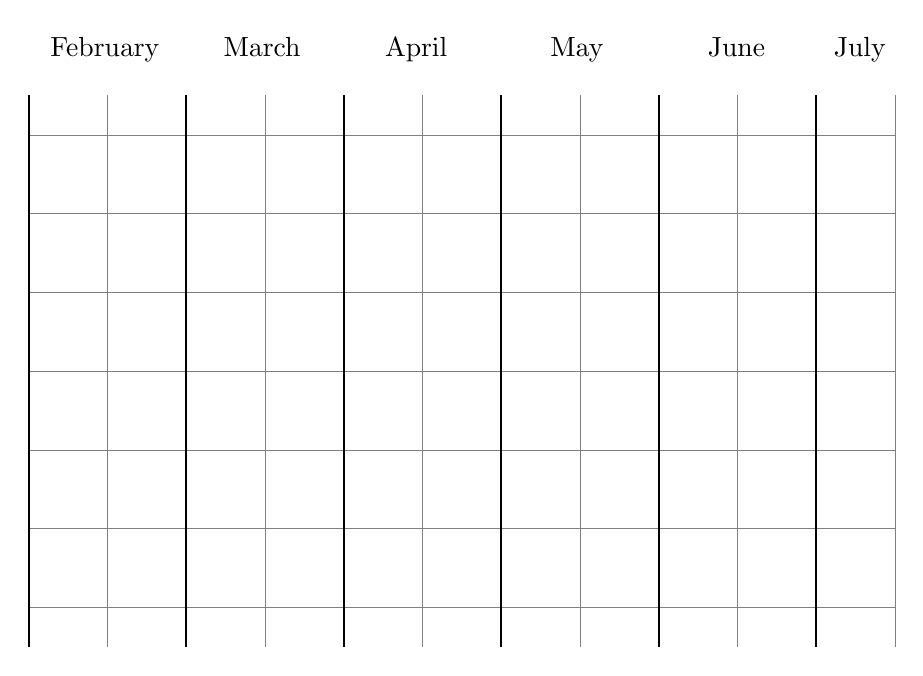
\begin{tikzpicture}[y=-1cm]
      \draw[help lines] (0,7.5) grid (11,0.5);
      \draw[thick] (0,0.5) -- (0,7.5);
      \draw[thick] (2,0.5) -- (2,7.5);
      \draw[thick] (4,0.5) -- (4,7.5);
      \draw[thick] (6,0.5) -- (6,7.5);
      \draw[thick] (8,0.5) -- (8,7.5);
      \draw[thick] (10,0.5) -- (10,7.5);
      
      \node at (0.15,0.0) [anchor=base west] {February};
      \node at (2.35,0.0) [anchor=base west] {March};
      \node at (4.4,0.0) [anchor=base west] {April};
      \node at (6.5,0.0) [anchor=base west] {May};
      \node at (8.5,0.0) [anchor=base west] {June};
      \node at (10.1,0.0) [anchor=base west] {July};
      
      \ganttline{1}{Operating Systems}{15}{30}
      \ganttline{2}{Web servers}{22}{37}
      \ganttline{3}{Ruby interpreters}{22}{55}
      \ganttline{4}{Databases}{22}{70}
      \ganttline{5}{Ruby on Rails}{22}{95}
      \ganttline{6}{Escolinhas}{22}{125}
      \ganttline{7}{Thesis Writing}{125}{155}
    \end{tikzpicture}
 
    \caption{Work scheduling}
    \label{fig:gantt}
  \end{center}
\end{figure}\\
All the mentioned testing, tuning, bottleneck research and improvements are directly related to scaling and performance optimizations, as suggested throughout this thesis.
Once again, it becomes critical to reaffirm that each area will be essentially targeted from the Rails perspective, taking sensitive dependences into account in order to avoid optimizing a specific component while taking the risk of making the system, as a whole, slower or less scalable.
\end{comment}

